\documentclass[master=cws,masteroption=gs]{kulemt}
\setup{title={Schaalbare genoomanalyse met NoSQL- databases},
		author={Brecht Gossel\'e},
		promotor={Prof. Dr. Roel Wuyts},
		assessor={},
		assistant={Prof. Dr. Roel Wuyts}}
\setup{filingcard,
		translatedtitle=,
		udc=,
		shortabstract={Here comes a very short abstract, containing no more than 500 words. \LaTeX\ commands can be used here.}}
		
\usepackage{url}
\usepackage{graphicx}
\usepackage{booktabs}
\graphicspath{ {afbeeldingen/} }
\usepackage{color}
\usepackage{listings}
\usepackage[final]{pdfpages}
\usepackage{lscape}
\lstset{basicstyle=\footnotesize, showspaces=false, keywordstyle=\color{blue}, stringstyle=\color[RGB]{26,196,8}}
\usepackage[pdfusetitle,colorlinks,plainpages=false]{hyperref}

\begin{document}

\begin{preface}
\end{preface}

\tableofcontents

\begin{abstract}
\end{abstract}


\mainmatter

\chapter{Inleiding}
\label{inleiding}

\section{Probleemstelling}

Wetenschappelijke vooruitgang heeft ervoor gezorgd dat de kost om genomen te sequencen het afgelopen decennium exponentieel gedaald is, sinds 2008 zelfs aan een hogere snelheid dan de evolutie volgens de wet van Moore \cite{wetterstrand_sequencing_cost}. Dit is duidelijk zichtbaar op de grafiek in figuur \ref{sequencing_cost}. In allerhande soorten biologisch, medisch en pharmaceutisch onderzoek worden dan ook genomen van meer en meer organismen gesequenced en dit genereert enorme hoeveelheden data. Ter illustratie: de \textit{whole genome sequencing pipeline} van het Broad Institute \cite{broad_institute}, een referentie in het veld, genereert bij het sequencen van 1 volledig menselijk genoom in de orde van 3TB aan tussentijdse data. Het eindresultaat is 50 GB gecomprimeerde data voor 1 menselijk genoom bij 50x \textit{coverage} (een maat voor de resolutie \cite{coverage_definition}). Naarmate genomen van miljoenen mensen en andere levende wezens geanalyseerd en opgeslagen worden, vereist deze evolutie steeds betere schaalbaarheid, responstijd, en parallellisering voor de opslag en verwerking van deze data.\\

Een logische stap is om deze problemen aan te pakken met grote verdeelde computersystemen, zogenaamde \textit{high performance computing systems} of \textit{supercomputers}. Het Exascience Life Lab van imec, Intel, Janssen Pharmaceutica en de 5 Vlaamse universiteiten verricht specifiek onderzoek naar de toepassing van supercomputers om het genoomsequencingproces te versnellen \cite{lifelab_bwa}\cite{exascience_life_lab}.\\
De snel toegenomen populariteit van webdiensten als sociale netwerken zadelde webservice-leveranciers op met een gelijkaardige explosie aan data. Om deze zogenaamde Big Data \cite{mashey1997big} adequaat te beheren, volstaan traditionele relationele DBMS niet meer. Daarom hebben grote webbedrijven zoals Google, Amazon en Facebook nieuwe opslagtechnieken ontwikkeld die voldoen aan de vereisten qua incrementele schaalbaarheid, lage responstijden en hoge beschikbaarheid \cite{baker2011megastore}. Dit heeft vele zogenaamde NoSQL ('Not only SQL') databases voortgebracht, die het rigide relationele datamodel inruilen voor betere schaalbaarheid en gemakkelijkere distributie van de data. Daarnaast is er ook de recentere opkomst van NewSQL-systemen: deze trachten de schaalbaarheid, distributie en fouttolerantie van NoSQL-systemen te combineren met het relationele datamodel en de bijhorende SQL-query interface en sterke garanties op gebied van concurrency en consistentie.

\begin{figure}[h!]
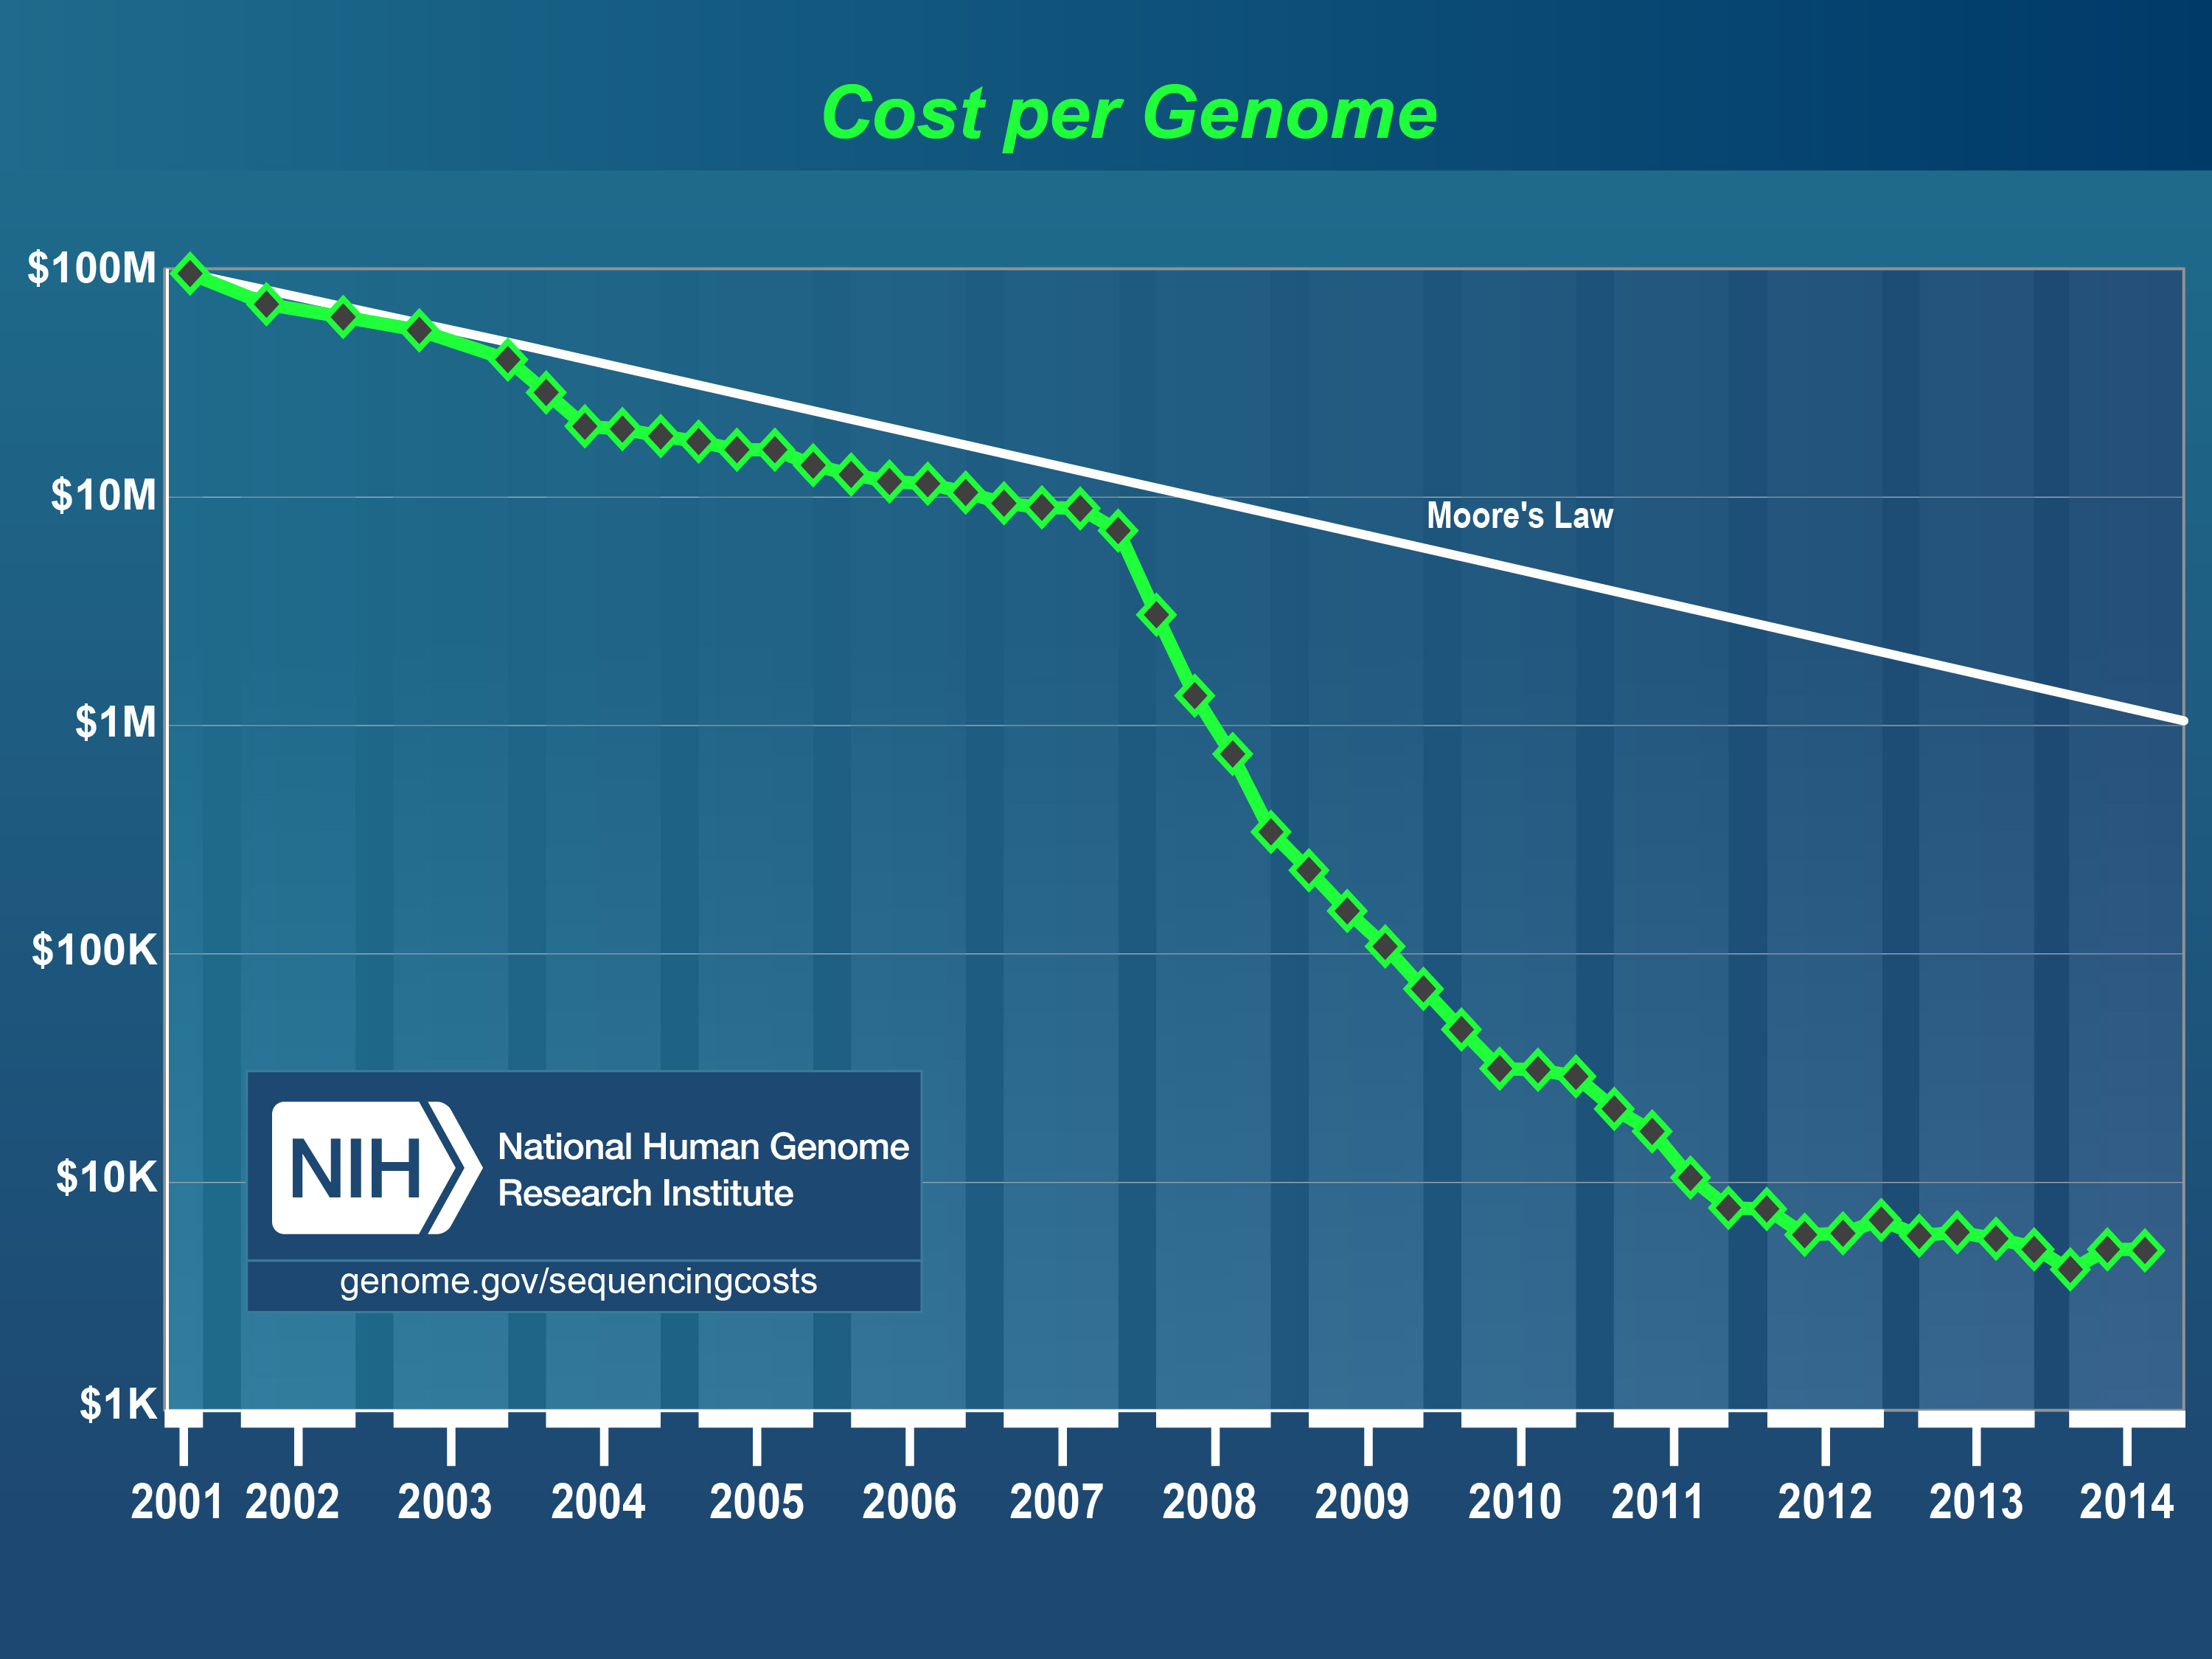
\includegraphics[width=\textwidth,height=\textheight,keepaspectratio]{cost_genome}
\caption{Evolutie van de prijs om een genoom te sequencen sinds 2001}
\label{sequencing_cost}
\end{figure}

\section{GEMINI}

Deze thesis bevat ook een case study over de opportuniteiten voor NoSQL-technologie\"en in de genoomanalysewereld. Op vraag van Janssens Pharmaceutica is het onderwerp hiervan de genoomanalysetool GEMINI (van GEnome MINIng): een software-framework voor flexibele analyse van genetische variaties in grote datasets van genomen, ontwikkeld aan de University of Utah \cite{10.1371/journal.pcbi.1003153}. GEMINI vertrekt daarbij van VCF (Variant Call Format) tekst-bestanden, laadt deze in in een database, voegt allerlei annotaties toe met bijkomende informatie van enkele vermaarde onderzoeksinstituten en biedt dan de mogelijkheid queries uit te voeren op deze databank. De huidige operationele versie van GEMINI draait op de eenvoudige SQL-databank SQLite, maar deze laat op gebied van schaalbaarheid en performantie te wensen over. De gewenste schaalbaarheid ligt in 2 dimensies: enerzijds het aantal genetische \textit{variants} in de dataset, d.w.z. stukken van genen zoals deze in het genoomsequencingproces waargenomen worden, en het aantal proefpersonen of \textit{samples} wier DNA in de dataset geanalyseerd wordt. Bij toenemend 
%TODO getal!
aantal samples of variants duurt zowel het inladen van de genoomdata in de databank voor als het queryen tijdens effectief gebruik te lang om gebruiksvriendelijk te zijn. Het inladen van de genoomdata uit VCF-files is, enigszins contra-intu\"itief, geen eenmalige of zeldzame operatie: de huidige productieversie van GEMINI laat niet toe om na het inladen nog samples of variants toe te voegen, met als gevolg dat bij elke iteratie van een genetisch of biologisch experiment die nieuwe informatie oplevert, de volledige dataset opnieuw ingeladen dient te worden. Ook het incrementeel kunnen toevoegen van variants en samples aan de gegevensset is dus een aandachtspunt bij het onderzoek naar mogelijke verbeteringen voor GEMINI.\\
Een eerste oplossing om de performantie te verhogen was om over te schakelen op PostgreSQL, en hiervan is intussen al met succes een eerste versie ge\"implementeerd. Het resultaat is een verhoging van de querysnelheden van 5 tot 20x, zonder verregaande optimalisaties. De verwachtingen zijn echter ook hier dat PostgreSQL op langere termijn niet zal kunnen schalen naar datasets van (honderd)duizenden genomen.\\
Naar de toekomst toe is het dus noodzakelijk uit kijken naar andere technologie\"en en types databanken om GEMINI ook bruikbaar te maken voor grootschaligere experimenten.

\section{Oplossing, contributies,...}

{\color{red} TODO}




\chapter{Achtergrond datastores}
\label{datastores_intro}

Sinds de jaren '70 zijn zogenaamde \textit{relational database management systems} (kortweg RDBMS) de voornaamste technologie voor de grootschalige opslag van gegevens. Ze zijn gestoeld op 2 belangrijke principes, namelijk het relationele datamodel \cite{codd1970relational} en de gestructureerde querytaal SEQUEL, beter gekend als SQL \cite{chamberlin1974sequel}. De architectuur van vele RDBMS is nog steeds gebaseerd op de eerste implementatie van een dergelijk systeem, namelijk het IBM onderzoeksproject System R \cite{blasgen1981system}, ook uit halverwege de jaren '70 \cite{Stonebraker:2007:EAE:1325851.1325981}. System R is uiteraard ontworpen voor destijds relevante hardwarekarakteristieken en productvereisten: business data processing via een command line interface, en dit op computersystemen met trage processoren, kleine werk- en schijfgeheugens maar relatief grote bandbreedte tussen de schijfopslag en het werkgeheugen. Dit leidde tot een aantal architecturale features die nog steeds terug te vinden zijn in hedendaagse RDBMS:
\begin{itemize}
\item Disk-geori\"enteerde opslag- en indexstructuren
\item Multithreading om latency op te vangen
\item Concurrency-controlemechanismen op basis van locking
\item Log-gebaseerd herstel van fouten
\end{itemize} 
Ondanks gigantische technologische vooruitgang op gebied van hardware en sterk gediversifieerde gebruiksscenario's, is er sinds hun ontstaan 40 jaar geleden weinig drastisch veranderd aan het concept van de RDBMS en zijn deze systemen de werkpaarden van de industrie geworden op het vlak van dataopslag.\\

Beginnende in de jaren 2000 groeide in de IT-wereld dan ook het besef dat de rigide \textit{one size fits all}-aanpak van RDBMS voor vele moderne toepassingen achterhaald dreigde te geraken. Met grote opkomende spelers uit de web-industrie zoals Google, Amazon en Facebook aan het roer leidde dit tot de opkomst van de NoSQL-beweging. NoSQL staat, in tegenstelling tot wat de naam doet vermoeden, voor \textit{Not only SQL} en omvat een waaier van uiteenlopende alternatieve gegevensopslagsystemen die elk in bepaalde specifieke opzichten meerwaarde trachten te bieden ten opzichte van het klassieke relationele systemen. In tegenstelling tot de 'Zwitsers zakmes'-aanpak van RDMBS, leggen ze zich toe op zeer gespecialiseerde toepassingsdomeinen en proberen daarin relationele systemen te overtreffen. Vaak betekent dit dat NoSQL systemen vele voor hun doel onnodig geachte features van SQL systemen achterwege laten, of afzwakken. Een goed voorbeeld hiervan zijn de ACID-eigenschappen uit het relationele model die in vele NoSQL-systemen gereduceerd zijn tot zogenaamde BASE-eigenschappen (op het verschil tussen beide komt sectie \ref{consistentie} nog uitgebreid terug).

De reden waarom web-spelers overstapten op NoSQL-systemen of er zelf ontwierpen, is voornamelijk dat deze geschikter zijn voor de enorme hoeveelheden data die dergelijke bedrijven sinds de opkomst van Web 2.0 moeten verwerken. NoSQL-systemen staan er om bekend horizontaal en incrementeel te schalen naar gigantische datasets: door eenvoudigweg servers toe te voegen aan de cluster onder de databank, en niet door bestaande servers up te graden (i.e. verticaal schalen), kan een cluster vlot meegroeien met de dataset. Bovendien draaien NoSQL-systemen doorgaans op goedkope commodity hardware, dus standaard servers, in plaats van dure gespecialiseerde databankservers. Goedkope doordeweekse servers laten toe om zowel kost- als energie-effici\"enter redundantie en dus ook fouttolerantie in te bouwen en zo de zeer hoge vereiste beschikbaarheid te garanderen \cite{barroso2003web}. NoSQL-systemen zijn bijgevolg grootschalige, gedistribueerde systemen, met bijhorende mechanismen om data ten eerste op te splitsen en te verspreiden (ook: partitioneren of sharden) en ten tweede te repliceren over de cluster. Replicatie heeft meerdere doelen: verhoogde bedrijfszekerheid, load balancing en verhoogde doorvoer in lees-intensieve toepassingen.

\section{Concepten}

Deze sectie belicht de belangrijkste begrippen in verband met NoSQL-databanken en contrasteert waar nodig met gelijkaardige concepten in het klassieke traditionele model.

\subsection{Partitionering}

Gezien de grote datahoeveelheden en gedistribueerde setting van NoSQL is het een noodzaak data in de databank te verspreiden. Er bestaan meerdere strategie\"en om de entries in een databank (dit kunnen rijen, documenten, simpele values,\ldots zijn) over de nodes in een cluster te verdelen. Ten eerste is er het onderscheid tussen horizontaal en verticaal partitioneren: bij horizontaal schalen, ook sharding genoemd, wordt een entry niet gefragmenteerd, maar in zijn geheel toegewezen aan een node, op basis van een op de entry gedefinieerde key. De meeste NoSQL datastores implementeren een versie van horizontaal partitioneren. Verticaal partitioneren stamt uit het relationele model, en betekent het splitsen van grote tabellen in meerdere kleinere tabellen.\\
Binnen het horizontaal partitioneren bestaan 2 voorname methodes \cite{grolinger2013data}:
\begin{itemize}
\item \textit{Range partitioning:} elke server is verantwoordelijk voor een bepaald bereik van key-waarden. Deze methode leent zich uitstekend tot het verwerken van range queries, gezien opeenvolgende keys vaak op eenzelfde node zullen liggen. Er is echter ook een belangrijk nadeel met deze aanpak verbonden: ze kan leiden tot load-balanceringsproblemen en \textit{hot spots}. Wanneer een applicatie bijvoorbeeld de gegevens in volgorde van hun key-waarden verwerkt, zal de werklast steeds bij dezelfde servers geconcentreerd liggen. Een ander nadeel is dat een centrale routing server de mapping van de ranges van keys naar nodes moet bijhouden, die dan client requests naar de juiste nodes door kan sturen. Dit introduceert een mogelijke flessenhals in het systeem.
\item \textit{Consistent hashing:} zoals de naam doet vermoeden, gebeurt de partitie in dit geval op basis van een hash van de key van entries. De output van de hash-functie wordt als een ring beschouwd en alle nodes krijgen een willekeurige waarde of positie toegewezen op deze ring. Een entry wordt dan toegewezen door via de hash van zijn key zijn positie in de ring te bepalen en vervolgens de ring klokwijs te bewandelen tot de eerste node met positie groter dan de positie van de entry. Het voordeel van consistent hashing is dat de positie van een object zeer snel berekend kan worden en dat hier geen centraal bewaarde mapping voor nodig is. Bovendien is het toevoegen van nodes zeer eenvoudig: enkel de buren van een nieuwe node op de ring merken dit, waardoor weinig entries verplaatst moeten worden. Een belangrijk nadeel is dat consistent hashing range queries bemoeilijkt, gezien opeenvolgende entries nu verspreid kunnen liggen over verschillende nodes.\\
Een techniek die vaak gepaard gaat met consistent hashing is het gebruik van \textit{virtual nodes} om load-balancing te verbeteren: elke fysieke node in de cluster krijgt meerdere posities toegewezen op de ring, en is zo verantwoordelijk voor meerdere virtuele nodes. Dit zorgt voor een betere verdeling van de entries over de nodes, gezien entries niet per se uniform over de ring verdeeld liggen. Bovendien moeten niet alle fysieke nodes verantwoordelijk zijn voor evenveel virtuele nodes: het systeem kan meer virtuele nodes toewijzen aan performantere fysieke nodes en zo rekening houden met heterogeniteit in de fysieke infrastructuur. Bovendien zal, bij het falen van een fysieke node, zijn opgeslagen last eerlijk verspreid worden tussen de overgebleven fysieke nodes. Omgekeerd zal een nieuwe node wanneer hij toetreedt tot de cluster van alle andere fysieke nodes ongeveer evenveel last overnemen  \cite{grolinger2013data}\cite{decandia2007dynamo}.
\end{itemize}  

\subsection{Consistentie}
\label{consistentie}

Consistentie van database-transacties betekent dat transacties de databank in een consistente staat achterlaten: alle data die een applicatie kan zien, is een consistente snapshot van de databank \cite{ports2010transactional}. Traditionele RDBMS bieden vaak transacties met de zogenaamde ACID-eigenschappen \cite{haerder1983principles}:
\begin{itemize}
\item \textbf{Atomicity:} Elke transactie gebeurt ofwel volledig, ofwel helemaal niet.
\item \textbf{Consistency:} Elke transactie laat de databank in consistente staat achter.
\item \textbf{Isolation:} Elke transactie verloopt volledig ge\"isoleerd van elke andere transactie en be\"invloedt deze dus op geen enkele manier.
\item \textbf{Durability:} Eens voltrokken, blijft elke transactie duurzaam bewaard in de databank, ook in het geval van stroomonderbrekingen, crashes of fouten.
\end{itemize}

Zoals Eric Brewer stelde in zijn bekende CAP-theorema \cite{brewer2000towards}, is het in een gedistribueerd systeem niet eenvoudig zowel consistentie, availability als tolerantie voor partities te bereiken en zijn 2 van deze 3 eigenschappen het hoogst haalbare\footnote{Brewer kwam hier zelf 12 jaar later op terug, stellende dat mits goede omgang met partities het toch mogelijk is een trade-off van alle drie te bereiken \cite{brewer2012cap}.}.
Ook in NoSQL-systemen, die vaak gedistribueerd van aard zijn, is het garanderen van consistentie geen triviale opgave. Afhankelijk van de gehanteerde schrijfstrategie is het mogelijk dat verschillende knopen in de cluster verschillende versies van data zien, als updates nog niet in de volledige cluster doorgekomen zijn. Daarom is er het onderscheid tussen strikte en uiteindelijke ("\textit{eventual}") consistentie: strikte consistentie is de gekende vorm waarin updates onmiddellijk zichtbaar zijn op alle nodes in de cluster, en dus ook naar bovenliggende applicaties toe. In het geval van uiteindelijke consistentie garandeert het systeem enkel dat na verloop van tijd alle nodes in de cluster dezelfde, up-to-date versie van de data zullen zien. NoSQL-systemen bieden dan ook vaak de BASE-eigenschappen, een zwakkere versie van de ACID-garanties:
\begin{itemize}
\item \textbf{Basically available:} Het systeem is onder quasi alle omstandigheden beschikbaar.
\item \textbf{Soft state:} Het systeem verkeert niet altijd in een consistente staat
\item \textbf{Eventually consistent:} Na verloop van tijd zal het systeem in een gekende staat verkeren.
\end{itemize}

Vele NoSQL-systemen stellen de gebruiker echter niet voor een voldongen feit bij de keuze tussen strikte en uiteindelijke consistentie: dankzij zogenaamde \textit{quora} kan de gebruiker zelf configureren welke consistentie het systeem levert. Door lees- en schrijfquora in te stellen, kan de gebruiker tunen hoeveel replica's respectievelijk moeten returnen bij een schrijfopdracht, en het welslagen van een schrijfopdracht moeten bevestigen. Op deze manier kan de gebruiker zelf een trade-off maken tussen snel lezen, schrijven en de behaalde consistentie. Bovendien zal de gebruiker, wanneer de som van het lees- en schrijfquorum groter is dan de replicatiefactor van de cluster, steeds de meest recente versie van gegevens zien, wat hetzelfde betekent als onmiddellijke, strikte consistentie.

\subsection{Storage layout}
\label{storage_layout}
Ook op het gebied van hoe ze gegevens zowel op schijf als in het geheugen opslaan, verschillen NoSQL-systemen van elkaar. Sommigen hanteren de gebalanceeerde B-bomen die ook vele RDBM-systemen gebruiken. Anderen, in navolging van Google Bigtable, doen beroep op zogenaamde \textit{log-structured merge trees}. In deze strategie worden updates niet onmiddellijk naar schijf geschreven: de data wordt in werkgeheugen aangepast en de update wordt op schijf gelogd. Wanneer er genoeg updates in geheugen gebeurd zijn, worden deze allemaal tegelijkertijd naar schijf geschreven. Dit kan sequentieel gebeuren, en vermijdt zo vele random writes, wat de schrijfdoorvoer uiteraard ten goede komt. 


\section{NoSQL-klassen}

NoSQL databanken zijn er in verschillende soorten en kunnen op basis van hun datamodel in een aantal categorie\"en onderverdeeld worden:

\begin{itemize}
\item \textbf{Key-Value stores} zijn vergelijkbaar met dictionaries en mappen unieke keys op values. Deze values zijn voor de databank volledig betekenisloze byte-arrays en de enige manier om ze op te vragen, is via de bijhoren key. Voor zeer eenvoudige toepassingen resulteert dit in hoge lees- en schrijf-throughput, maar meer geavanceerde features zoals indexing, queries, en het modelleren van relaties binnen de data zijn hierdoor niet mogelijk\cite{hecht2011nosql}\cite{grolinger2013data}.

\item \textbf{Columnar stores}
\label{Bigtable} zijn gebaseerd op het datamodel dat Google's Bigtable heeft ge\"introduceerd en slaan data op in een spaarse, gedistribueerde, persistente en multidimensionele gesorteerde map\cite{chang2008bigtable}. In het geval van Bigtable zijn dit drie dimensies: row key, column key en een timestamp. Bigtable is voorzien op de enorme hoeveelheden data die Google op dagelijkse basis verwerkt en de hiervan afgeleide columnar stores staan dan ook bekend om hun uitstekende schaalbaarheid. De goede schaalbaarheid en fouttolerantie van Bigtable is ook deels toe te schrijven aan het onderliggende gedistribueerde file systeem, Google File System \cite{ghemawat2003google}. Andere innovaties uit Bigtable zijn onder andere het gebruik van log-structured merge trees (zie \ref{storage_layout}) en Bloom filters: een effici\"ent probabilistische mechanisme om te voorspellen of een object in een verzameling zit (in dit geval, of een key in een tabel ligt, wat het aantal nodeloze table scans beduidend kan inperken) \cite{mullin1983second}.\\
Omdat net als in Key-Value stores het systeem hier de opgeslagen data niet interpreteert, is het modelleren van relaties niet op een effici\"ente manier mogelijk. Dit wordt overgelaten aan de bovenliggende applicatie \cite{hecht2011nosql}.

\item \textbf{Document stores} bewaren data als key-value paren en encapsuleren deze in documenten. Values kunnen van een brede waaier aan types zijn, zoals geneste documenten, lijsten of scalars. De namen van attributen kunnen dynamisch gespecifieerd worden tijdens runtime en moeten geen vooraf vastgelegd schema volgen\cite{cattell2011scalable}. Dit is geschikt voor het modelleren van ingewikkelde datastructuren. Vele document stores gebruiken het JSON-bestandsformaa (of een daarvan afgeleide vorm). In tegenstelling tot columnar stores, zijn de waarden in documenten niet betekenisloos voor het document store systeem en het is dus mogelijk hier indexen op te defini\"eren en queries op uit te voeren \cite{hecht2011nosql}.

\item \textbf{Graph databases:} zoals de naam doet vermoeden, stammen ze uit grafentheorie en maken ze gebruik van grafen als datamodel. Ze zijn uitermate geschikt om sterk verweven data te beheren, van bronnen zoals sociale netwerken of location based services. Hiervoor doen ze beroep op effici\"ente mechanismen om grafen te doorlopen waar andere systemen kostelijke operaties als recursieve joins gebruiken\cite{hecht2011nosql}.

\end{itemize}

De term NewSQL slaat op een verzameling systemen die ambi\"eren het klassieke relationele datamodel te combineren met de schaalbaarheid, distributie en fouttolerantie van NoSQL systemn. Hoewel ze allen de gebruiker het relationele model en SQL-achtige query mogelijkheden bieden, verschillen NewSQL stores onderling grondig, afhankelijk van de onderliggende architectuur. Zo zijn er onder meer systemen die gebouwd zijn bovenop bestaande NoSQL databanken, en andere die alle data in main memory opslaan.\cite{grolinger2013data}

\section{NoSQL: vergelijkende studie}
\label{nosql_survey}

Op de vraag of NoSQL en NewSQl-systemen al dan niet geschikt zijn om het genoomanalyseproces schaalbaarder te maken, bestaat geen eenvoudig antwoord. Gezien de grote diversiteit in de beschikbare gegevensopslagsystemen, zullen sommige systemen onvermijdelijk beter geschikt zijn dan andere, of beter geschikt voor andere aspecten van de genoom-analyse pipeline. Een vergelijkende studie van NoSQL- en NewSQL-systemen dringt zich dus op. Deze sectie bekijkt 6 systemen in meer detail en licht toe hoe ze van pas zouden kunnen komen in de genoomanalyse.

\subsection{Methodologie}

Omwille van het enorme aanbod aan NoSQL en NewSQL systemen was een exhaustieve studie niet haalbaar. Deze vergelijkende studie behandelt de populairste datastores in een aantal relevante categorie\"en, namelijk document stores, columnar stores en NewSQL stores. Key-value stores en graph databases komen niet aan bod, aangezien hun datamodellen niet geschikt zijn voor de toepassing in kwestie. De uiteindelijke selectie werd gemaakt volgens criteria vergelijkbaar met die in \cite{grolinger2013data}, met de ranking van DB-Engine Ranking \cite{db_engine_rank} als maat voor de populariteit.\\

\begin{landscape}
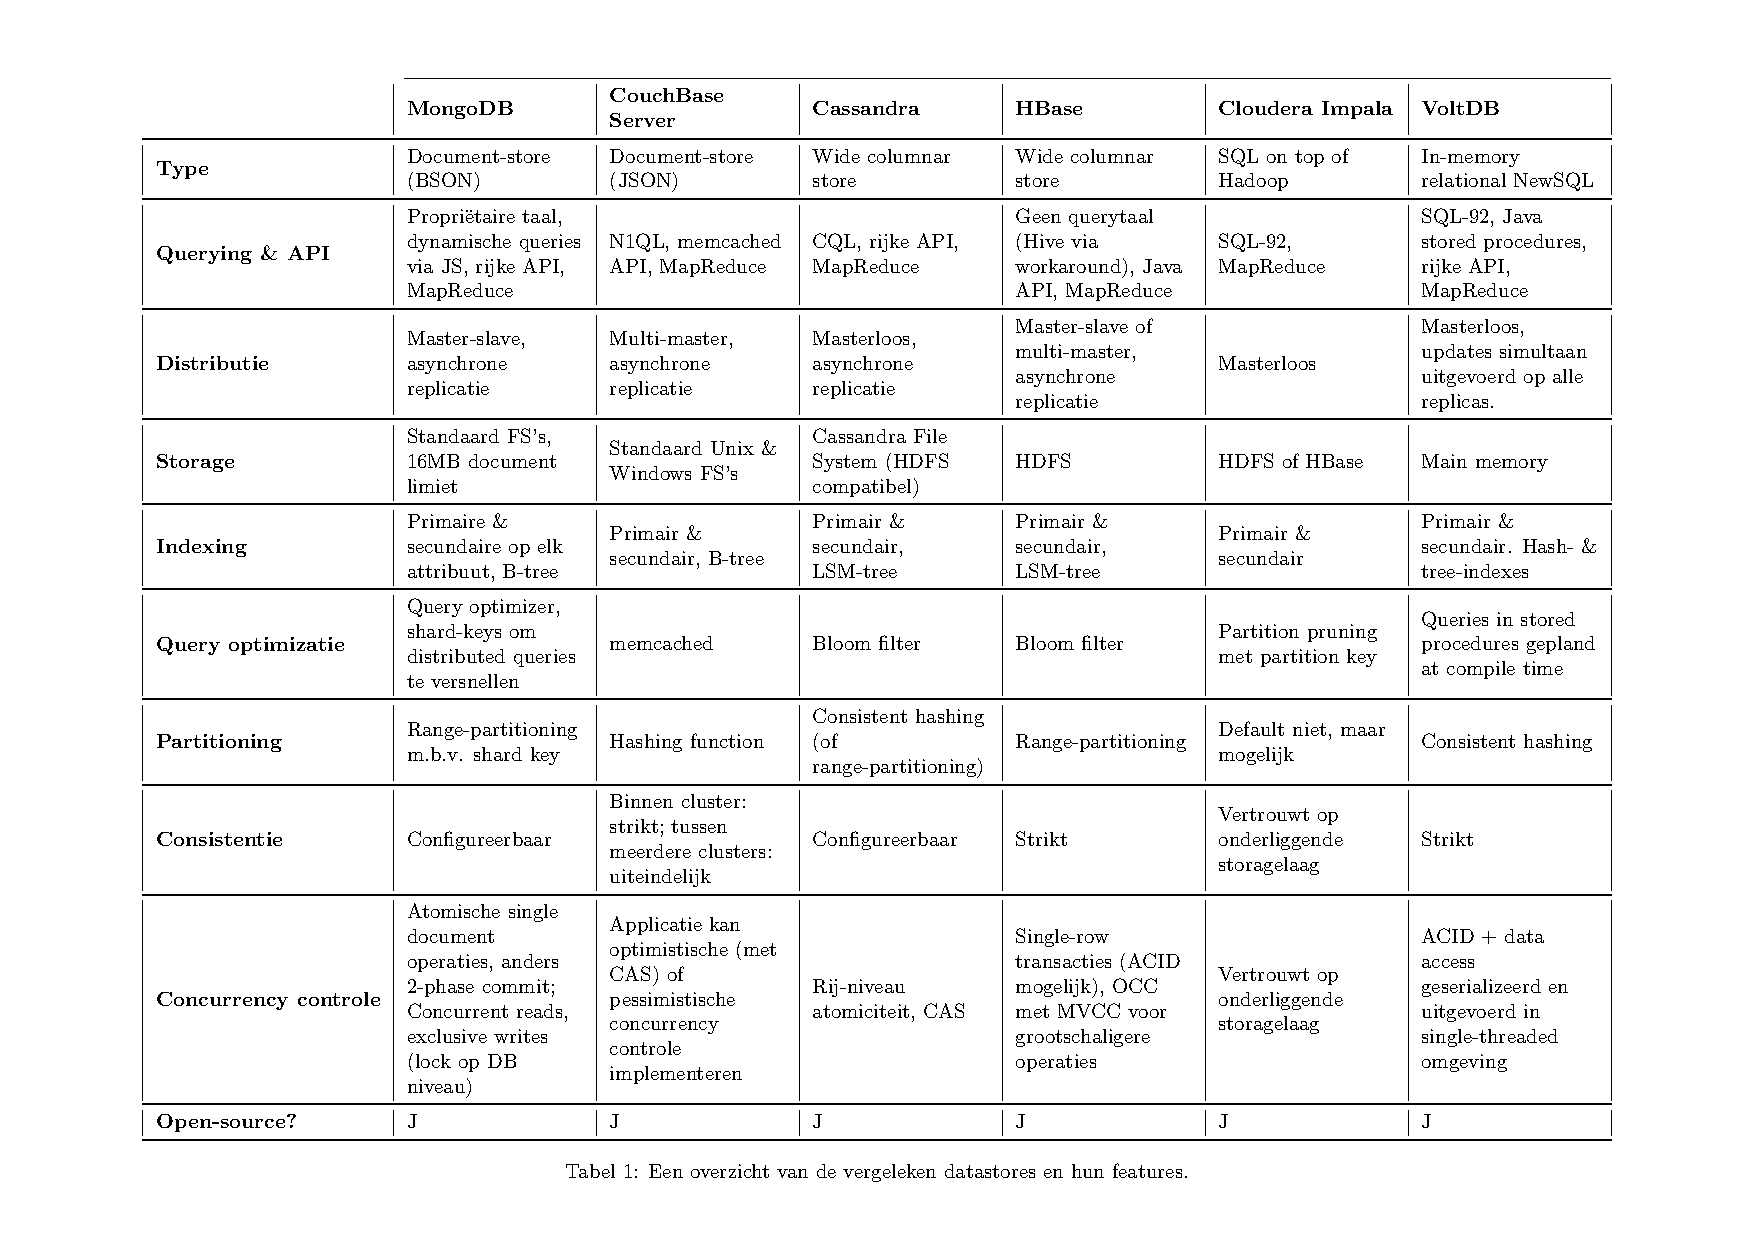
\includepdf[angle=90]{NoSQL_table_nl.pdf}
\label{survey_tabel}
\end{landscape}

Deze ranglijst tracht populariteit te meten op basis van enkele parameters, zoals aantal vermeldingen op websites, algemene interesses volgens Google Trends, frequentie van technische discussies op fora zoals StackOverflow, vacatures i.v.m. de technologie en vermeldingen in professionele profielen op sites zoals LinkedIn. De resulterende selectie bestaat uit de document stores MongoDB en CouchBase Server, wide columnar stores Cassandra en HBase en NewSQL database VoltDB. Er bestaat al een uitbreiding van de DNA sequencing pijplijn die het ExaScience Life Lab gebruikt om MongoDB  databanken als in- en/of uitvoer te gebruiken voor de pijplijn. Dit maakt MongoDB uiteraard nog relevanter. Ten laatste werd ook NewSQL query engine Cloudera Impala in de studie betrokken wegens expliciete interesse van onderzoekers in het eerder vernoemde lab.

\noindent Deze 6 systemen vergeleken we vervolgens op een aantal voor high performance computing relevante eigenschappen zoals indexeringsmechanismen, interfaces naar de gebruiker en API's, distributiestrategie, concurrency controle en consistentiemodel. Tabel \ref{survey_tabel} geeft een overzicht weer van de bestudeerde systemen.

\subsection{Document stores}

\subsubsection{MongoDB}

MongoDB slaat gegevens op in BSON (binary JSON) documenten. Het systeem biedt krachtige ondersteuning voor indices, vooral door de mogelijkheid om secundaire indices van een brede waaier van types te defini\"eren op alle attributen, zoals in het relationele model. Deze indices zijn gebouwd op B-trees \cite{mongodb_indexes}. Om denormalizatie te bevorderen, kunnen documenten geneste documenten en arrays bevatten. Zo zijn joins ook overbodig in de query taal.\\
De bestandsgrootte is beperkt tot 16 MB, om te voorkomen dat \'e\'en enkel document buitensporig veel RAM of bandbreedte opeist. Om grotere bestanden te bewaren, kan het ingebouwde GridFS (dat integenstelling tot wat de naam doet vermoeden, geen volwaardig file system is) automatisch bestanden opsplitsen in kleinere delen en deze delen als aparte documenten bewaren, zonder dat de gebruiker zich hierom moet bekommeren.\\
MongoDB biedt API's in zeer vele programmeertalen en de functionaliteit om het equivalent van SQL \texttt{WHERE}-clausules te defini\"eren als javascript uitdrukkingen. MongoDB vertaalt deze vervolgens naar een eigen, interne en afgeschermde query taal \cite{grolinger2013data}. De query optimizer van MongoDB verwerkt queries en kiest voor elke query een zo effici\"ent mogelijk uitvoeringsplan gegeven de beschikbare indices. Deze plannen worden gecached als er meerdere goede alternatieven zijn en kunnen geherevalueerd worden naarmate de gegevensset in de databank evolueert.\\
Qua consistentie laat MongoDB de keuze tussen uiteindelijke en strikte consistentie. Strikte consistentie is mogelijk door ofwel enkel te lezen van de master node (die de meest up-to-date versie van de data heeft) of na schrijfopdrachten te wachten tot alle replica's bevestigd hebben alvorens verder te gaan. De eerste optie introduceert een bottleneck bij het lezen van data, de tweede verhoogt de latentie van schrijfopdrachten.\\
MongoDB repliceert data asynchroon en partitioneert in ranges: nodes zijn verantwoordelijk voor ranges van keys. Dit zorgt voor snelle range queries, maar kan hotspots en load-balancingproblemen veroorzaken. Dankzij een master-slave struktuur kan MongoDB updates gemakkelijk naar de juiste replica's doorverwijzen.
Op het gebied van concurrency controle biedt MongoDB atomiciteit binnen documenten en reader-writer locks. Bij schrijfopdrachten de databank locken heeft een zware impact op de performantie in scenario's waar veel geschreven moet worden.\\\\
Kortom, MongoDB bewaart BSON-bestanden op een zeer toegankelijke manier met flexibele query- en indexeringsmechanismes. De concurrency- en consistentiemodellen daarentegen vertonen enkele nadelen.

\subsubsection{Couchbase Server}

Couchbase, het resultaat van de fusie tussen CouchDB en Membase, slaat gegevens op in JSON documenten. Het hanteert het memcached protocol om een gedistribueerde cache en is bedoeld voor zeer interactieve toepassingen met hoge vereisten op gebied van latentie \cite{grolinger2013data}\cite{couchbase_about}.
De JSON documenten kunnen genest zijn en kunnen doorzocht worden met een uitgebreide, SQL-achtige taal, N1QL (op het moment van schrijven is dit wel nog steeds een developer preview, uitgebracht in januari 2015) \cite{couchbase_n1ql}.
Net als MongoDB kunnen primaire en secundaire indices gedefinieerd worden en zijn deze gestoeld op B-trees \cite{couchbase_index}.\\
Binnen \'e\'en cluster zijn transacties strikt consistent, maar tussen meerdere clusters slechts uiteindelijk consistent.\\
CouchBase biedt gebruikers de keuze tussen optimistische (m.b.v. compare-and-swap) en pessimistische (m.b.v. 'finegrained locking') concurreny controle.\\\\
Dankzij zijn flexibele datamodel, caching en concurrency controle, past CouchBase goed voor toepassingen die snelle en intensieve interactieve vergen tussen gebruiker en data.

\subsection{Columnar stores}

\subsubsection{Cassandra}

Cassandra werd oorspronkelijk ontwikkeld voor intern gebruik bij Facebook maar is later als Apache opensourceproject publiekelijk beschikbaar gemaakt. Het combineert het columnaire datamodel van Google's Bigtable systeem (zie \ref{Bigtable}) met de architectuur en distributiestrategie van Amazons DynamoDB. Het is gericht op flexibele, quasipermanent beschikbare opslag van zeer grote datasets op goedkope standaardhardware, met daarenboven hoge througput voor schrijfopdrachten zonder effici\"entie bij leesopdrachten op te offeren \cite{borthakur2011apache}.\\
Sinds zijn ontstaan is Cassandra wel op enkele vlakken afgeweken van het BigTable-model \cite{cassandra_then&now}, in die zin dat het nu tabellen en \textit{composite columns} biedt, evenals een eigen query taal, CQL \cite{cassandra_CQL}. CQL vertoont op het gebied van syntax en functionaliteit sterke gelijkenissen met SQL, maar is toch sterk beperkt. Zo biedt het bijvoorbeeld geen \texttt{JOIN}-clausule, en zijn \texttt{WHERE}-clausules aan sterke voorwaarden onderhevig. Cassandra moedigt het samen bewaren van gegevens die samen opgevraagd worden sterk aan en ondersteunt denormalizatie met features zoals collection types.\\
Cassandra heeft indexeringsmechanismes and implementeert deze met log-structured merge trees, met hogere schrijfthroughput als gevolg. Ook biedt Cassandra net als Google Bigtable Bloom filters.\\
Om lineair in het aantal ingeschakelde nodes te kunnen schalen naar zeer grote datasets, opereert Cassandra op een volledig hi\"erarchieloze wijze. Vanuit het perspectief van het CAP-theorema, spitst Cassandra zich toe op availability en partition tolerance, ten koste van onmiddellijke consistentie. Het consistentieniveau kan wel per query door de gebruiker bepaald worden, zoals later verduidelijkt wordt. Hoge beschikbaarheid en tolerantie voor fouten bereikt Cassandra door asynchroon data te repliceren over verschillende nodes, met consistent hashing en virtuele nodes om frequent komen-en-gaan en incrementeel toevoegen van nodes op te vangen. Het aantal replica's kan de gebruiker zelf kiezen. Bovendien voorziet Cassandra ook interdatacenterreplicatie, om zelfs het falen van volledige datacenters op te vangen \cite{decandia2007dynamo} \cite{lakshman2010cassandra} \cite{cassandra_then&now}.\\
Bij lees- en schrijfopdrachten kan de gebruiker een quorum specifi\"eren. Hoewel Cassandra met uiteindelijke consistentie voor het oog ontworpen werd, is onmiddellijke consistentie mits een juiste keuze van de quorum dus ook een optie.\\
Op het gebied van concurrency controle garandeert Cassandra atomiciteit binnen rijen en serializeerbare \textit{lightweight transactions}, eigenlijk compare-and-set functionaliteit, voor grotere operaties.
\\\\
Samengevat biedt Cassandra redelijk flexibele datamodellering met (licht beperkte) query- en indexeringsmechanismen via de CQL-interface. Het sterkste punt is echter dat Cassandra incrementeel schaalt naar enorme datasets, dankzij uitvoerige replicatie- en foutverwerkingsfeatures.

\subsubsection{HBase}

Apache HBase is een opensource datastore gebaseerd op Google Bigtable, die draait bovenop het Hadoop Distributed File System (HDFS) in plaats van het Google File System (GFS).\\
Sinds z'n lancering heeft HBase verschillende secundaire indexeringsmechanismes verworven. Deze zijn ook gebaseerd op LSM trees en daarnaast biedt ook HBase Bloom filters \cite{borthakur2011apache}\cite{hbase_schema}. HBase heeft een Java API, maar zonder SQL-achtige geavanceerde querytaal. Hierbij moet wel opgemerkt worden dat een omweg via Apache Hive, een ander data-opslag en -analyseproject \cite{apache_hive}, en de bijhorende querytaal HiveQL dit probleem kan verhelpen. Dankzij de HDFS-fundering can HBase vlot fungeren als in- en output voor MapReduce taken.\\
HBase partitioneert data net als Bigtable in ranges en repliceert gegevens op ofwel master-slave of multi-master wijze. Leesopdrachten worden echter niet gedistribueerd: er is slechts 1 server die instaat voor elke rij. De replica's zijn enkel bestemd voor het herstellen van fouten.\\
De sterke punten van HBase zijn de sterke consistentie, een rariteit in de NoSQL-wereld, en concurrency-model: ACID transactions binnen rijen en optimistische, multi-version concurrency controle voor grootschaligere operaties \cite{hbase_acid}\cite{grolinger2013data}\cite{borthakur2011apache}.\\

Kort samengevat laat HBase gebruikers toe flexibel data te modelleren en is het systeem vooral nuttig wanneer het startpunt een dataset in HDFS is en MapReduce-compatibiliteit een prioriteit is. HBase schaalt goed naar zeer grote datasets en beschikt over uitstekende concurrency- en consistentie-eigenschappen.

\subsection{NewSQL} 

\subsubsection{VoltDB}

VoltDB is een relationele, gedistribueerde in-memory databank, die als doel heeft de garanties van klassieke SQL-stores te koppelen met de schaalbaarheid van NoSQL-systemen, en bovendien aan zeer hoge snelheden te functioneren \cite{stonebraker2013voltdb}.\\
VoltDB bewaart gegevens in het traditionele relationele model, maar gerepliceerd en gepartitioneerd (met consistent hashing) over verschillende nodes \cite{grolinger2013data}. De data is doorzoekbaar via een (groeiende) subset van SQL-92 \cite{voltdb2010voltdb}. Queries worden bij voorkeur gedefinieerd als stored procedures in Java, met daarin ingebed de SQL uitdrukkingen. Gezien de queries dan op voorhand gekend moeten zijn, leent VoltDB zich dus ook niet optimaal tot flexibele ad-hoc queries. VoltDB ondersteunt primaire en secundaire indices en laat de gebruiker de keuze tussen hash- en boomindices \cite{voltdb_indexes}. VoltDB plant en optimaliseert de queries in stored procedures offline tijdens het compileren \cite{voltdb_query_plans}.\\
Omdat VoltDB volledig op RAM geheugen vertrouwt, is het duur om te schalen naar datavolumes in de grootorde van meerdere petabytes, maar VoltDB kan data exporteren naar andere, meer geschikte databanksystemen zoals columnaire NoSQL systemen.\\
Vooral op het gebied van concurrency controle onderscheidt VoltDB zich van andere systemen: transacties voldoen aan de ACID-eigenschappen en worden simultaan op alle replica's uitgevoerd. Het geheugen is in blokken verdeeld, die elk statisch toegewezen zijn aan \'e\'en enkele, single-threaded core. Een globale controller serializeert alle transacties waarbij meerdere nodes betrokken zijn tot een sequentie van enkelvoudige transacties en voegt deze in de transaction queues van de betrokken nodes. Op deze manier maakt VoltDB locking en latching technieken overbodig. De durability uit ACID bereikt VoltDB door op regelmatige basis snapshots van de databank in het geheugen te nemen en deze op schijf op te slaan.\\

Kort samengevat is VoltDB een relationele databank in main memory die schaalt tot relatief grote datasets, met zeer snelle SQL-query-capaciteiten en ACID-transacties. Het is bijgevolg meer geschikt voor rekenintensieve toepassingen die niet overdreven veel data verwerken, maar wel zeer lage latentie vereisen.

\subsubsection{Cloudera Impala}

Cloudera Impala is een gedistribueerde SQL-machine die draait bovenop de Hadoopstack, ofwel op HDFS of op HBase \cite{cloudera_impala}. Ze is specfiek bedoeld voor analytisch gebruik, met een focus op het leveren van real-time query-capaciteiten eerder dan op hoge throughput bij schrijfopdrachten.\\
Opgeslagen data is toegankelijk via een subset van SQL-92.\\
Impala's architectuur is bijna perfect symmetrisch gedistribueerd: alle nodes voeren hetzelfde \texttt{impalad}-proces uit, dat de belangrijkste databankfunctionaliteiten verzorgt. Elke node kan als startpunt fungeren voor een query en zal vervolgens de query in kwestie co\"ordineren. Twee processen lopen daarentegen op \'e\'en enkele (niet noodzakelijk dezelfde) node in de cluster; zij staan in voor boekhoudkundige taken en doorgeven van wijzingen aan metadata doorheen de cluster \cite{impala_components}.\\
In tegenstelling tot voorgaande opties partitioneert Impala rijen niet automatisch. De gebruiker krijgt wel de keuze hiertoe, voor in het geval de hoeveelheid gegevens hierom zou vragen \cite{impala_partitioning}.\\
Impala beschikt over een zeer effici\"ente I/O-laag die schijf- en CPU-gebruik te allen tijde hoog houdt, wat resulteert in aanzienlijk snellere prestaties dan andere SQL-on-Hadoop oplossingen zoals Apache Hive \cite{floratou2014sql}. Het inherente nadeel is echter dat de volledige dataset moet passen in het totale werkgeheugen van de cluster waarin Impala draait. Dit beperkt enigszins de grootte van datasets diet Impala kan verwerken, ondanks de schaalbaarheid van de onderliggende Hadooplaag.\\
Omwille van z'n analytische doeleinden heeft Impala geen uitvoerige mechanismes voor concurrency controle, maar vertrouwt hiervoor op het onderliggende opslagsysteem. Gezien de uitstekende concurrency-eigenschappen van HBase vormt dit niet noodzakelijk een probleem.

\subsection{Vergelijkende studie: conclusies}

Deze sectie bestudeerde 6 datastores, 2 van de populairste in 3 verschillende categorie\"en, en vergeleek ze met elkaar op een een aantal eigenschappen relevant voor HPC toepassingen. Columnaire stores als Cassandra en HBase zijn geschikt om gigantische datasets op te slaan op een robuuste en performante manier, en zouden kunnen dienen om de informatie uit reeds gesequencete genomen op te slaan. MongoDB blinkt uit dankzij een uitgebreide API, flexibele datamodel, en query- in indexeringsmechanismen. Het beschikt niet over even goede schrijfeigenschappen als de columnaire systemen, maar is desondanks een sterke kandidaat voor de opslag van grote datasets zoals genomen. VoltDB en CouchBase Server bieden lage latency bij lees- en schrijfopdrachten, zij het op kleinere datasets, maar lenen zich dus goed tot het bewaren van snel evoluerende tussentijdse gegevens in de sequencing pipeline. Tot slot is Cloudera Impala geschikt voor situaties waar snelle, mogelijks ingewikkelde leesqueries eerder dan schrijfqueries op grote datasets vereist zijn. Ook Impala is dus eerder geschikt voor de analyse van al gesequencete genomen, maar op kleiner schaal dan de columnaire NoSQl-databanken.

\section{Achtergrond datastores: conclusies}

Dit hoofdstuk schetst de belangrijkste technologische achtergrond van deze thesis op het gebied van databanksystemen. NoSQL en NewSQL kunnen, dankzij hun afkomst uit de webwereld, geschikt zijn om om te gaan met de grote hoeveelheden data die de bioinformatica met zich meebrengt. Na een toelichting van enkele essenti\"ele begrippen zoals consistentie, partitionering en storage layout, kwam een vergelijkende studie van 6 NoSQL en NewSQL-systemen aan bod, met specifieke aandacht voor hoe elk van deze systemen van toepassing kan zijn in de genoomanalysepijplijn.


\chapter{GEMINI overzicht}
\label{gemini_beschrijving}

Zoals eerder vermeld is GEMINI een applicatie voor de flexibele analyse van genoomdata van populaties van menselijke individu\"en. Deze sectie gaat dieper in op de belangrijkste features en het onderliggende datamodel van GEMINI in zijn oorspronkelijke vorm \cite{10.1371/journal.pcbi.1003153}\cite{gemini_docs}.

\section{Database schema}

GEMINI importeert genetische variants en genotypes van alle gesampelde individu\"en (ook 'samples') vanuit een VCF file in een relationele database.
Daarnaast kan extra informatie over de samples, zoals geslacht, phenotype en onderlinge verwantschappen, meegegeven worden in een PED-file (van pedigree) om latere analyse te vergemakkelijken.\\

Elke variant in een input VCF file wordt uitvoerig geannoteerd na automatische vergelijking met bestaande of door de gebruiker gedefinieerde genoom-annotatiebestanden. De geannoteerde variants vormen de rijen van de hoofdtabel van de database, de \texttt{variants}-tabel. Deze tabel bevat ook voor elke variant informatie over elke sample, zoals diens genotype, de kwaliteit en diepte van de meting voor de variant in kwestie. In de SQLite-versie van GEMINI wordt dit opgeslagen als een gecomprimeerde array per variant, 1 voor elke sample-eigenschap: zo is er een \texttt{gt\_type}-kolom met arrays met de genotypes, en een \texttt{gt\_depth}-kolom met arrays met de diepte van de meting van elke sample voor elke variant. Samen met de \texttt{samples}-tabel, die voor elke sample zaken als het geslacht, phenotype en familierelaties bijhoudt, ligt de \texttt{variants}-tabel aan de basis van de uitgebreide query-mogelijkheden die GEMINI biedt.\\

Daarnaast zijn er nog tabellen zoals de \texttt{variant\_impacts}- en \texttt{gene\_detailed}-tabellen die respectievelijk extra informatie over de variants en het menselijk genoom bevatten. Deze informatie komt in het eerste geval eveneens uit de annotatiebestanden, en in het tweede uit tekstbestanden met referentie-informatie over het menselijk genoom die GEMINI, indien gewenst mee inlaadt.\\
Ten laatste zijn er nog enkele kleine tabellen met meta-informatie, zoals de \texttt{resources}-tabel die de gebruikte annotatie-files bevat, en de \texttt{version}-tabel die bevat door welke versie van GEMINI de data ingeladen is.\\

Een belangrijke troef van GEMINI en z'n datamodel is de flexibiliteit die het laat naar de gebruiker. Zo kan de gebruiker zelfgedefinieerde annotatie-files gebruiken, en zelf kolommen toevoegen aan de PED-files met informatie over de samples. Deze extra informatie zal GEMINI automatisch in de resp. \texttt{variants}- en \texttt{samples}-tabel opnemen en kan de gebruiker later ook doorzoeken.

\begin{figure}[h]
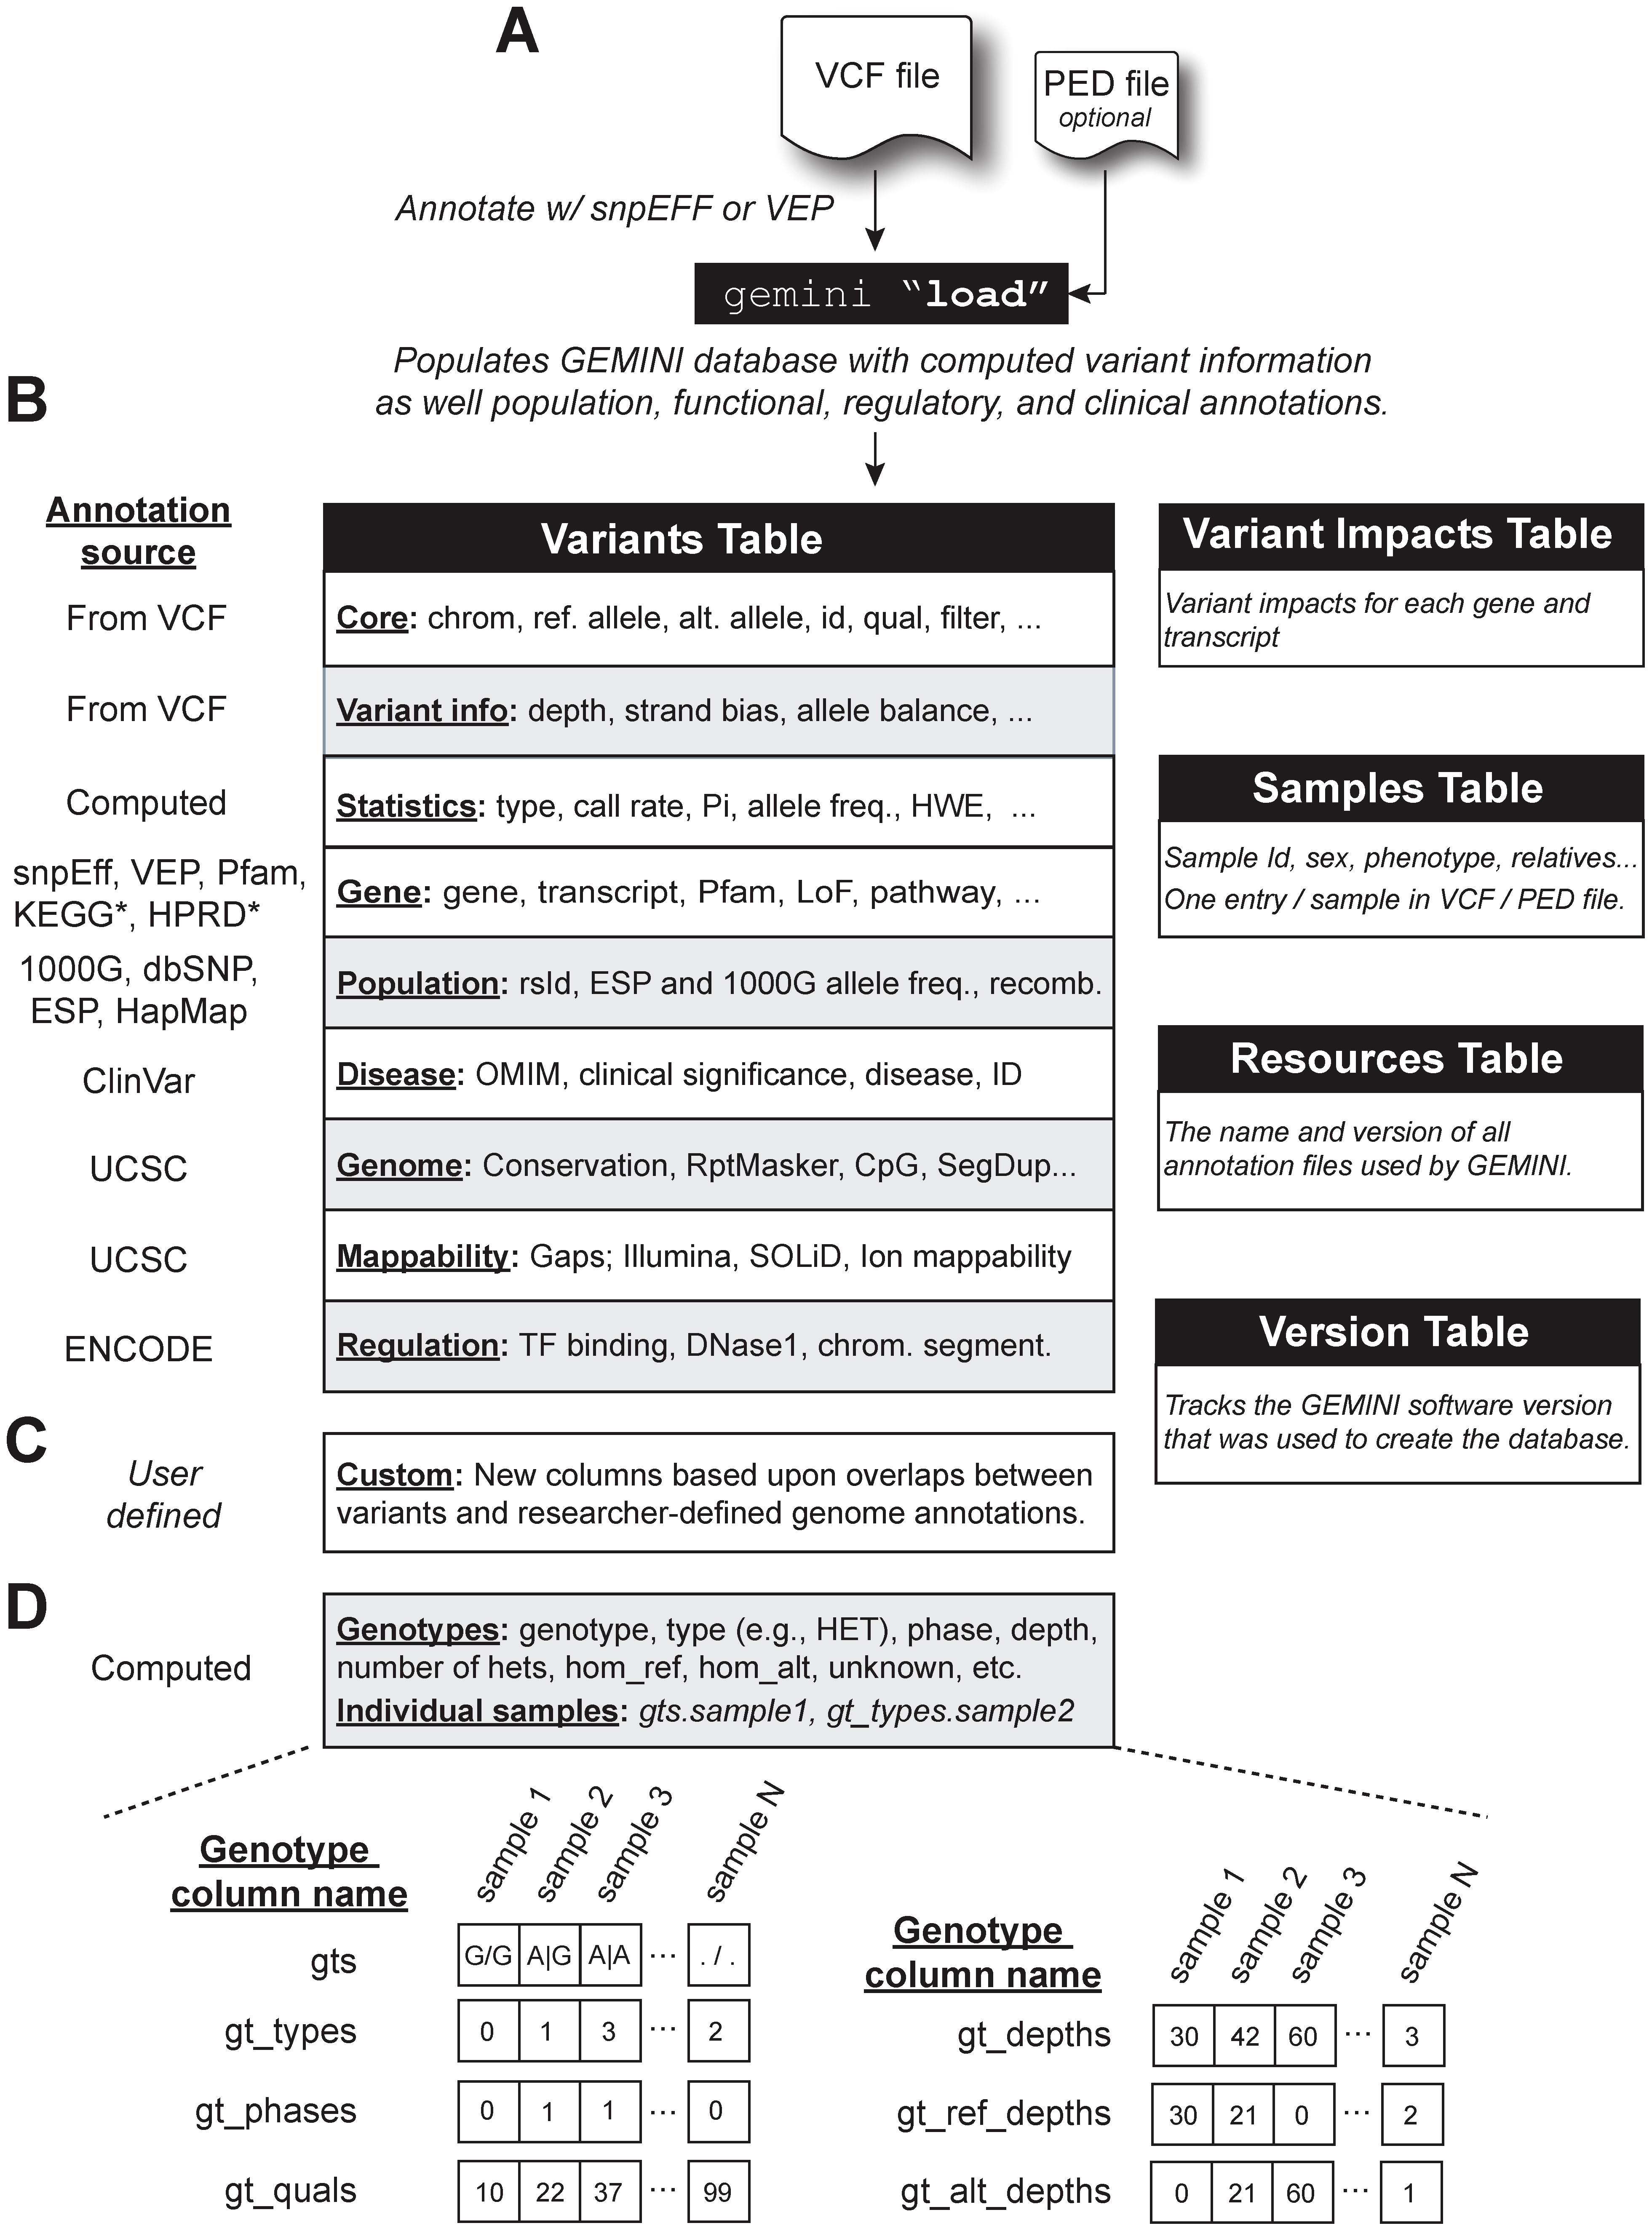
\includegraphics[width=\textwidth,height=\textheight,keepaspectratio]{gemini_schema}
\caption{Een overzicht van GEMINI's schema}
\label{gemini_schema_pic}
\end{figure}

\section{Inladen}
Het inladen van de data uit VCF-bestanden is een computationeel intensieve operatie, enerzijds omwille van de enorme grootte van deze bestanden, en anderzijds omdat in deze fase ook alle variants geannoteerd moeten worden. Om het proces te versnellen, biedt GEMINI de mogelijkheid het werk te paralleliseren door het VCF-bestand de comprimeren, op het bestaande bestand een index te defini\"eren en zo het werk te verdelen. Dit kan over meerdere processoren binnen 1 computer zijn, maar via de IPython-interface ook over volledige clusters van computers \cite{PER-GRA:2007}.\\

\section{Querying}

GEMINI laat de gebruiker toe de opgeslagen genoomdata te doorzoeken. Enerzijds via gewone SQL-queries, maar omdat het onderzoeken van individuele genotypes van cruciaal belang is in het onderzoek naar ziektes en SQL standaard niet de individuele genotypes in array-kolommen kan opvragen, biedt GEMINI bovendien een verrijkte SQL-syntax.\\
Zo laat het de gebruiker toe via filters en wildcards de gewenste genotype-eigenschappen en samples te specifi\"eren.

\subsection{Sample filters/wildcards} 
In SQL \texttt{SELECT}-statements kan de gebruiker met een filter van de vorm column.sample of een wilcard van de vorm (column).(wildcard) uitdrukken welke genotype-kolommen van welke samples hij/zij wilt zien. Wanneer de gebruiker ge\"interesseerd is in bijvoorbeeld het genotype van Jan, wordt dit:\\
\texttt{SELECT gt\_types.Bob FROM variants}\\\\
Als de gebruiker de diepte van de genotypes alle vrouwelijke samples wil zien, wordt dit:\\\\
\texttt{SELECT (gt\_depths).(sex = 'female')}.\\
GEMINI vertaalt de wildcard automatisch naar een query op de \texttt{samples}-tabel, en kan vervolgens voor alle samples die aan de voorwaarden voldoen, de waarde uit de gevraagde kolom tonen.

\subsection{Genotype filters/wildcards}
Om beperkingen op te leggen aan de variants waarin hij ge\"interesseerd is, kan de gebruiker SQL \texttt{WHERE}-clausules uitbreiden met zogenaamde genotype filters. Is de gebruiker bij voorbeeld enkel ge\"interesseerd in variants waarvoor Bob heterozygoot is en Bruce alles behalve heterozygoot is, kan dit met:\\

\noindent\texttt{\$ gemini query -q} "\texttt{SELECT * FROM variants}"\textbackslash \\\texttt{--gt-filter }"\texttt{gt\_types.Bob == HET and gt\_types.Bruce != HET}"\\

\noindent Vaak is het de bedoeling om eenzelfde beperking op te leggen aan meerdere samples. Op bovenstaande manier wordt dit al monikenwerk. Om dit te verhinderen, zijn er genotype wildcards van volgend formaat:\\ 
\texttt{(column).(sample\_wildcard).(gt\_wildcard\_rule).(rule\_enforcement)}.
\begin{description}
\item[column] Staat voor de genotype kolom waarop de beperking slaat.
\item[sample\_wildcard] Een wildcard om aan te duiden voor welke samples de beperking moet gelden. Analoog met de eerder vermelde sample wildcards.
\item[gt\_wildcard\_rule] De beperking op de genotype kolom.
\item[rule\_enforcement] Duidt aan hoeveel van de geselecteerde samples aan de opgelegde gt\_wildcard\_rule moeten voldoen. Dit kan \texttt{all, any, none, of count <comparison>} zijn.
\end{description}

\noindent Alle variants opvragen waarvoor alle mannen heterozygoot zijn, gaat bijvoorbeeld met:

\noindent\texttt{\$ gemini query -q "}\texttt{SELECT * FROM variants"}\textbackslash \\
\texttt{--gt-filter" }\texttt{(gt\_types).(sex = 'male').(=HET).(all)"}\\

\noindent Alle variants opvragen waarvoor minstens 1 bruinharig individu een genotype van diepte minstens 100 heeft, met:

\noindent\texttt{\$ gemini query -q "}\texttt{SELECT * FROM variants"}\textbackslash \\
\texttt{--gt-filter" }\texttt{(gt\_depths).(hair\_colour = 'brown').(>=100).(any)"}\\

\noindent Alle variants opvragen waarvoor minder dan 10 individu\"en een genotype met diepte minder dan 50 hebben, met:

\noindent\texttt{\$ gemini query -q "}\texttt{SELECT * FROM variants"}\textbackslash \\
\texttt{--gt-filter" }\texttt{(gt\_depths).(*).(=HET).(count < 10)"}\\

\noindent Al de bovenstaande filters kunnen met elkaar gecombineerd worden, evenals met gewone WHERE-clausules op de andere kolommen van de variants-tabel.

\subsection{\texttt{--show-samples}}

GEMINI biedt ook de mogelijkheid, bij een query op de \texttt{variants}-tabel, voor elke variant die aan de gestelde eisen voldoet, de namen van alle samples weer te geven die voor gegeven variant homozygoot of heterozygoot zijn. Dit gebeurt door de \texttt{--show-samples} flag mee te geven aan het \texttt{query} commando.




\chapter{Cassandra \& GEMINI: implementatie}
\label{implementatie}

Dit hoofdstuk beschrijft de praktische realisatie van een versie van GEMINI draaiende op Cassandra in de plaats van SQLite, verderbouwend op het ontwerp uit hoofdstuk \ref{concept}. De implementatie is gebaseerd op versie 0.1.11 van GEMINI, 2.1.4 van Apache Cassandra en versie 2.5.1 van de Python driver voor Cassandra, ontwikkeld door DataStax \cite{cassandra_driver}. 

\section{\texttt{gemini load} met Cassandra}
Het inladen van genoomdata in GEMINI gebeurt in twee stappen. De reden voor die opsplitsing is dat een klein deel van het inladen en initialiseren van de databank niet parallel op meerdere processoren kan verlopen. \\In de eerste en kleinste van de twee, initialiseert GEMINI de databank, maakt de nodige tabellen aan en laadt de samples-informatie in. GEMINI haalt de namen van de samples uit de VCF-file, en vult die aan met informatie uit de PED-file. Indien er geen PED-file voorhanden is, initialiseert GEMINI de \texttt{samples}-tabel met default-waarden voor de kolommen zoals \texttt{sex} en \texttt{phenotype}. Meteen worden ook de extra, aan de \texttt{samples}-tabel verbonden tabellen zoals \texttt{samples\_by\_sex} en \texttt{samples\_by\_phenotype} aangemaakt en gevuld. Ook de \texttt{resources-, gene\_detailed-, gene\_summary-} en \texttt{version-}tabellen worden in de eerste fase gevuld. Dit omdat de pedigree-files en de bestanden met data over de genen niet effici\"ent opgesplitst kunnen worden. Bovendien is de duur van het inladen van de \texttt{samples}-tabel zelfs bij 10000'en samples verwaarloosbaar tegenover het inladen en annoteren van de \texttt{variants}-tabel.\\
In de tweede fase gebeurt het leeuwendeel van het werk: het inladen van de variants-informatie uit de (verplicht meegegeven) VCF-file. Dankzij de bgzip \cite{bgzip} en grabix \cite{grabix} tools kan GEMINI effici\"ent VCF-bestanden in blokken opsplitsen, comprimeren, hierop een index defini\"eren en vervolgens daarmee verderwerken. Zo kan GEMINI eenvoudig het inladen van de variants, die elk \'e\'en lijn in de VCF-file in beslag nemen, gemakkelijk over meerdere cores verdelen. Het is ook in deze fase dat GEMINI de aan de \texttt{variants}-tabel verwante tabellen zoals \texttt{variants\_by\_samples\_gt\_type}, \texttt{variants\_by\_samples\_gt\_depth} en \texttt{variants\_by\_chrom\_start} opvult. Alle cores of nodes in het cluster, voeren rechtstreeks rijen in in \'e\'en en dezelfde tabel in de Cassandra-databank. Omdat Cassandra atomiciteit binnen rijen garandeert en alle workers strikt disjuncte sets van variants invoeren in het systeem, is er geen enkel risico op conflicten.\\\\
De grote winst ten opzichte van de SQLite-implementatie van GEMINI is dat in het parallelle gedeelte, alle workers naar dezelfde databank kunnen schrijven. In de SQLite-versie van GEMINI schrijven alle workers naar een aparte SQLite-database, die vervolgens in een kostelijke operatie nog allemaal samengevoegd moeten worden tot \'e\'en grote SQLite-databank. Die stap (het \texttt{gemini merge}-commando) kan de Cassandra-implementatie volledig overslaan. Een ander opzicht waarin de Cassandra-implementatie effici\"enter is dan de SQLite-versie, is dat in SQLite voor elke variant de genotype-kolommen nog tot binary blobs gecomprimeerd worden. In Cassandra is dit, dankzij de keuze van het databaseschema, niet nodig.

\section{\texttt{gemini query} met Cassandra}
\label{gemini_query_impl}

\subsection{Splitsing in subqueries}


Om zoals in het voorbeeld uit \ref{splitsing_subqueries_conceptueel} dynamisch beslissingen over het splitsen in subqueries te kunnen maken, is het nodig de \texttt{WHERE}-clausule te inspecteren en hieruit de benodigde hulptabellen voor de subqueries te identificeren. Om dit proces te vereenvoudigen, hanteert deze implementatie een licht gewijzigde querysyntax: beperkingen die binnen 1 hulptabel liggen, kunnen nog steeds met elkaar gecombineerd worden met het \texttt{AND}-keyword, maar beperkingen die niet binnen eenzelfde hulptabel liggen, moeten met de \texttt{\&\&, ||} of \texttt{NOT}-operatoren van elkaar gescheiden worden. Zo kan GEMINI bij het parsen van de \texttt{WHERE}-clausule deze onmiddellijk opsplitsen in subqueries en voor elk van deze subqueries de nodige hulptabel bepalen. Beschouw wederom volgende query:\\\\
\texttt{SELECT chrom, start, subtype FROM variants WHERE chrom = 'chromX' \\AND start > 5600 AND gene = 'gene\_A'}.\\\\
In de aangepaste syntax wordt dit:\\\\
\texttt{SELECT chrom, start, subtype FROM variants WHERE chrom = 'chromX' \\AND start > 5600 \&\& gene = 'gene\_A'}.\\

Dit vereist uiteraard dat de gebruiker op de hoogte is van welke hulptabellen er bestaan. Gebruikers moeten sowieso weten op welke kolommen ze queries kunnen defini\"eren, en bijgevolg ook welke hulptabellen er bestaan. Bovendien bestaat het doelpubliek van GEMINI uit onderzoekers die het programma intensief gebruiken en dus voldoende gelegenheden hebben om dergelijke aanpassingen snel onder de knie te krijgen.\\
%TODO
Een andere optie is de syntax onveranderd te laten en uit de in de \texttt{WHERE}-clausule vermelde kolommen benodigde hulptabellen af te leiden. Die aanpak heeft als voordeel dat de interface naar de gebruiker niet verandert, maar gezien nog steeds enkel queries mogelijk zijn op kolommen uit de hoofdtabel waarvoor hulptabellen bestaan, is achterwaartse compatibiliteit hiermee nog niet verzekerd. Daarbovenop levert ze ook nieuwe problemen op, zoals: wat met kolommen die in meerdere hulptabellen voorkomen, welke combinatie van tabellen wordt er dan best geselecteerd? Dergelijke vraagstukken neigen naar query-optimization en vallen buiten het ... {\color{red} TODO} Daarom verkoos ik de macht bij de gebruiker te leggen en te vertrouwen op diens oordeelkundigheid.\\\\
De gebruiker dient er ook rekening mee te houden dat Cassandra range-queries enkel onder strikte voorwaarden ondersteunt, namelijk (zoals eerder uitgelegd) enkel op clustering columns en enkel wanneer de voorgaande kolommen in de clustering key met gelijkheden beperkt zijn. Dit impliceert dat er slechts een range query op 1 kolom in een tabel mogelijk is. Daarnaast biedt Cassandra ook geen \texttt{!=}-operator. Dit euvel valt te verhelpen door een \texttt{!=}-clausule om te zetten naar een gelijkheidsbeperking en die vervolgens te negeren. Een clausule als \texttt{phenotype != 2} wordt dan \texttt{NOT (phenotype = 2)}. Dit vereist dat de \texttt{!=}-clausule een aparte subquery vormt.\\

Het uiteindelijke algoritme om de geschikte hulptabel te selecteren op basis van de kolommen en gebruikte operatoren in een subquery, gebruikt de metadata van het Cassandra-cluster om alle hulptabellen voor een gegeven hoofdtabel op te vragen, en vervolgens aan de hand van de kolommen in de primary keys van de kandidaat-hulptabellen de geschikte eruit te kiezen.\\

GEMINI encapsuleert de subqueries in \texttt{query\_expression}s: een set Python-klassen die, ge\"inspireerd door algebra\"ische datatypes uit functionele talen zoals Haskell, alle mogelijke GEMINI-queries kunnen voorstellen. Die bevatten alle informatie die GEMINI nodig heeft om de queries te evalueren. De \texttt{Basic\_expression} stelt een eenvoudige query op een Cassandra-tabel voor. Tijdens het parsen van de \texttt{WHERE}-clausule zal GEMINI de subqueries inkapselen in \texttt{Basic\_expressions} en die, afhankelijk van de gehele query, nesten in \texttt{AND\_}-, \texttt{OR\_}- of/en \texttt{NOT\_expression}s. De \texttt{GT\_wildcard\_expression} stelt op een effici\"ente manier genotype-filter wildcards voor (zie \ref{gt_wildcards}). De volgende paragraaf bespreekt in detail de aangeboden \texttt{evaluate}- en \texttt{can\_prune}-functies.

\begin{figure}[h]
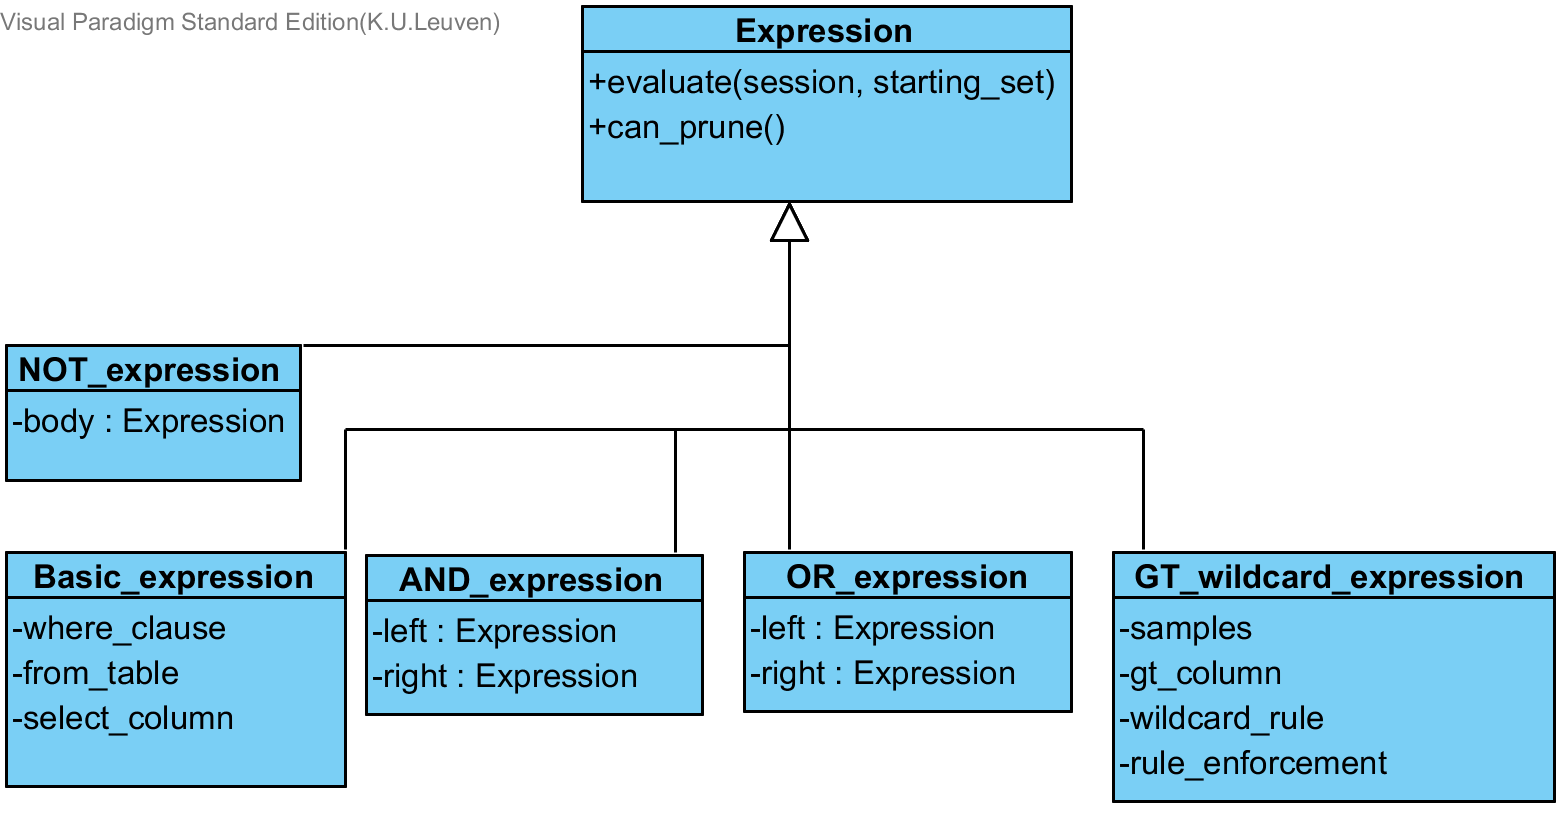
\includegraphics[width=\textwidth,height=\textheight,keepaspectratio]{query_exps}
\caption{De \texttt{query\_expressions} waarmee alle queries gemodelleerd worden. Het \texttt{session}-argument van de \texttt{evaluate}-functie is een actieve verbinding met het Cassandra-cluster.}
\label{query_exps_diagram}
\end{figure}

\subsection{Combineren subqueries}

Uit performantie-overwegingen is het een logische keuze de resultaten van subqueries op de hulptabellen te bewaren in een set datatype. Zo kunnen de benodigde set-operaties gebruik maken van de in Python ingebouwde set-operaties en zo veel effici\"enter verlopen dan wanneer de resultaten in bijvoorbeeld lists bewaard worden. Het enige nadeel van sets t.o.v. lists is dat de implementatie geen garanties biedt over in welke volgorde rijen in het eindresultaat zullen voorkomen. Dit weegt niet op tegen de tijdswinst, en bovendien biedt Cassandra zelf (in de algemeen aangeraden consistent hashing-partitionering) geen enkele garantie over in welke volgorde het rijen opslaat.\\\\
Bij het praktisch evalueren van \texttt{query\_expression}s komt uiteindelijk meer kijken dan enkel set-operaties. De belangrijkste reden hiervoor is dat, zoals in \ref{comb_subq_concept} reeds beschreven, om een negatie of \texttt{NOT\_expression} te kunnen evalueren, alle kandidaat-rijen gekend moet zijn, en dus meegegeven aan de \texttt{evaluate}-functie. Die extra informatie kan ook bij het evalueren van andere types van \texttt{query\_expression} goed van pas komen.
 
\begin{itemize}
\item Het evalueren van \texttt{Basic\_expression}s gebeurt niet zo rechtoe rechtaan als de naam doet vermoeden. De \texttt{evaluate}-functie bouwt een CQL-query op, op basis van een gegeven \texttt{WHERE}-clausule, de relevante tabel en de gevraagde kolom uit die tabel. Wanneer er een zinvolle verzameling kandidaatrijen (de \texttt{starting\_set} in onderstaand codefragment) meegegeven is, wordt die als \texttt{IN}-clausule aan de \texttt{WHERE}-clausule toegevoegd. Zo zoekt Cassandra enkel in rijen die effectief in aanmerking komen om aan de globale query te voldoen. Een voorwaarde om die optimalisatie te kunnen toepassen, is dat de \texttt{WHERE}-clausule geen ongelijkheidsbeperkingen mag bevatten (vandaar de \texttt{can\_prune}-functie).

\lstinputlisting[language=Python,firstline=31,lastline=48]{gemini_src/query_expressions.py}

\item Om een \texttt{AND\_expression} te evalueren is het strikt genomen nodig beide leden van de uitdrukking te evalueren en vervolgens de doorsnede te nemen van de resultaten. Als \'e\'en van de twee leden van de uitdrukking echter in staat is om dankzij een CQL \texttt{IN}-clausule enkel naar rijen te zoeken die effectief in aanmerking komen om aan de globale query te voldoen, is het mogelijk om die operatie aan Cassandra over te laten. Als het rechterlid kan \textit{prunen}, dan kan GEMINI de resultaatverzameling van het linkerlid als \texttt{starting\_set} meegeven bij de evaluatie van het rechterlid, en omgekeerd. Wanneer geen van beide kunnen \textit{prunen}, moet GEMINI uiteraard nog steeds zelf de doorsnede berekenen.

\lstinputlisting[language=Python,firstline=56,lastline=66]{gemini_src/query_expressions.py}

\item In het geval van een \texttt{OR\_expression} is er geen andere mogelijkheid dan eenvoudigweg het linker- en rechterlid te evalueren, beide met als \texttt{starting\_set} de \texttt{starting\_set} van de \texttt{OR\_expression} zelf, en vervolgens de unie van de resultaten te berekenen.

\item Ook in het geval van een \texttt{NOT\_expression} is er geen andere optie dan de \texttt{body}-uitdrukking te evalueren en vervolgens het complement van de \texttt{starting\_set} en het resultaat te bepalen. Als de gegeven \texttt{starting\_set} gelijk is aan \texttt{"*"}, d.w.z. alle rijen in de oorspronkelijke tabel, zit er ook niets anders op dan die nog eerst allemaal op te vragen.

\lstinputlisting[language=Python,firstline=101,lastline=110]{gemini_src/query_expressions.py}

\end{itemize}

Een optimalisatie die voor alle \texttt{query\_expressions} geldt is dat in het geval van een lege \texttt{starting\_set}, GEMINI de hele evaluatie kan overslaan. Dit bespaart een overtollige round-trip naar de Cassandra-databank. Voor alle soorten \texttt{query\_expressions} behalve \texttt{Basic\_expression} geldt ook dat ze kunnen \textit{prunen}, ongeacht de aard van hun subqueries. In het geval dat hun subqueries een \texttt{Basic\_expression} bevatten die niet kan \textit{prunen}, zal de subquery in kwestie dit zelf afhandelen bij de evaluatie.

\subsection{Genotype-filter wildcards}
\label{gt_wildcards}

Gegeven het bovenstaande query-mechanisme is de meest voor de hand liggende manier om genotype-filter wildcards te implementeren, ze op te splitsen in subqueries voor elke sample die aan de voorwaarden in de \texttt{sample\_wildcard} voldoet, en die subqueries te combineren met een keten van geneste \texttt{query\_expression}s afhankelijk van de gegeven \texttt{rule\_enforcement}. Zo wordt een \texttt{all}-wildcard een keten van geneste \texttt{AND\_expression}s en een \texttt{any}-wildcard een keten van geneste \texttt{OR\_expression}s. \texttt{none}-wildcards vereisen eerst dat de subqueries in \texttt{NOT\_expression}d ingebed worden, die vervolgens allemaal in een keten van geneste \texttt{AND\_expression}s gecombineerd worden. Het is moeilijker \texttt{count}-wildcards tot dergelijke \texttt{expressions} om te vormen. Die vergen een aparte strategie, die later aan bod komt.\\
Deze aanpak is vergelijkbaar met wat er in de SQLite- en PostgresQL-versies van GEMINI gebeurt: in SQLite vormt GEMINI de wildcards om tot lange Python-expressions die uiteindelijk voor elke variant met de Python \texttt{eval()}-functie ge\"evalueerd worden. Dit uiteraard omdat de genotype-kolommen bestaan uit binary blobs die voor de SQLite-databank geen enkele betekenis hebben. De PostgreSQL-versie van GEMINI pakt het slimmer aan en vormt de wildcards om tot lange SQL \texttt{WHERE}-clausules en laat zo het evaluatiewerk over aan de databank, met de bemerking dat de PostgreSQL-versie \texttt{count}-wildcards vooralsnog niet ondersteunt omdat dit niet rechtstreeks in SQL vertaald kunnen worden.\\
In dit opzicht lijkt de Cassandra-implementatie op de SQLite-implementatie, gezien de client, niet de databank, het meeste werk verricht.\\

Zoals in de conceptuele uitleg van de oplossing aangehaald, kan de evaluatie van genotype-wildcards effici\"enter verlopen door de evaluatie van de subqueries in parallel uit te voeren op meerdere processoren. Dit heb ik ook daadwerkelijk ge\"implementeerd, door introductie van een nieuw type \texttt{query\_expression}, namelijk de \texttt{GT\_wildcard\_expression}.\\
Bij evaluatie zal die de namen van alle samples die aan de \texttt{sample\_wildcard} voldoen verdelen over het aantal processoren dat de gebruiker meegeeft, elke processor een tussenresultaat laten berekenen, de resultaten opvragen en samenvoegen m.b.v. de gekende setalgebra. Om het werk effici\"ent over verschillende processoren te verdelen en alle benodigde informatie te communiceren, maakt de implementatie gebruik van zogenaamde subprocesses, die elk hun eigen verbinding openen met het Cassandra-cluster, en interprocess-communicatiemechanismen uit de Python \texttt{multiprocessing}-API \cite{multiprocessing}.\\

\lstinputlisting[language=Python,firstline=173,lastline=197]{gemini_src/query_expressions.py}

\texttt{all-, any-} en \texttt{none-}wildcards vereisen voor het samenvoegen van de resultaten van de verschillende subprocesses geen grote aanpassingen aan de sequenti\"ele evaluatie-strategie van wildcards. Omdat die oplossingswijze er zich uitstekend toe leent af te wijken van het stramien van de geneste \texttt{query\_expressions} (immers, er is maar 1 \texttt{GT\_wildcard\_expression} voor alle samples), is het makkelijker de \texttt{count}-wildcards te implementeren: elk subprocess voert subqueries uit voor de samples waarvoor het verantwoordelijk is en telt voor elke variant hoe vaak hij in de resultaatverzamelingen van de subqueries voorkomt. Die informatie stuurt het subprocess terug naar zijn parent-process in een Python \textit{dictionary}, met een map van \texttt{variant\_id}s naar de telling.

\lstinputlisting[language=Python,firstline=315,lastline=341]{gemini_src/query_expressions.py}

Het parent-process kan vervolgens de telling voor alle variants van alle subprocesses bij elkaar optellen, en met gebruik van de Python \texttt{eval}-functie alle variants die aan de \texttt{count}-filter voldoen, bepalen. Let wel, bij het opstellen van de uiteindelijke \textit{dictionary} met de tellingen voor de varianten, moet het parent-process voor alle varianten in de \texttt{starting\_set}, een entry voorzien, met defaultwaarde 0. Zoniet zullen varianten waarvoor geen enkele sample aan de \texttt{gt\_wildcard\_rule} voldoet, niet in het resultaat voorkomen, en \texttt{count}-filters als \texttt{(count < x), (count <= x)} (voor arbitraire, positieve \texttt{x}) of \texttt{(count == 0)}  die varianten onterecht niet in hun resultaat weergeven.

\lstinputlisting[language=Python,firstline=212,lastline=222]{gemini_src/query_expressions.py}

\noindent De \texttt{correct\_starting\_set} in bovenstaande code is de traditionele \texttt{starting\_set}, maar ge\"evalueerd in het geval dit de volledige verzameling varianten (dus de wildcard \texttt{"*"}) is, en gegoten in een datatype geschikt voor shared-memory access.\\
De \texttt{invert\_count}-flag geeft aan of de \texttt{gt\_wildcard\_rule} een negatie is. Gezien Cassandra geen \texttt{!=}-clausules ondersteunt, moet GEMINI in dit geval het complement van de \texttt{gt\_wildcard\_rule} in kwestie bepalen en vervolgens de resulterende telling aftrekken van het totaal aantal samples. \\ Een eenvoudig voorbeeld: bij het evalueren van volgende wildcard \\\\ 
\texttt{(gt\_type).(*).(!=HET).(count > 100)}\\\\
zal GEMINI eerst voor elke variant bepalen hoeveel samples w\'el heterozygoot zijn, alvorens dit getal af te trekken van het totaal aantal samples en op dit resultaat de \texttt{(count > 100)}-filter toe te passen.

\section*{Implementatie: conclusie}

De implementatie van het ontwerp beschreven in hoofdstuk \ref{concept} vergt vooral ingrijpende wijzigingen aan het queryingmechanisme van GEMINI: ons ontwerp analyseert queries at runtime, splitst \texttt{WHERE}-clausules en genotype-filters en -wildcards op in meerdere subqueries tegen de Cassandra databank en combineert de resultaten van die subqueries tot een coherent resultaat met behulp van set-arithmetiek. De evaluatie van de subqueries kan in parallel gebeuren op meerdere processoren om het gehele proces sneller te laten verlopen.\\
Aan het mechanisme om genoominformatie in te laden in GEMINI verandert er minder. Ook die taak kan dankzij Cassandra eenvoudig geparalleliseerd worden, door meerdere processoren los van elkaar een disjunct deel van de data in te laten laden, rechtstreeks in dezelfde Cassandra databank.

\chapter{Experimenten}
\chapter{Evaluatie}
\chapter{Future work}
\chapter{Conclusies}

\bibliographystyle{abbrv}
\bibliography{biblio}
\end{document}